\documentclass[tikz,border=6pt]{standalone}
\usepackage{tikz}

\begin{document}

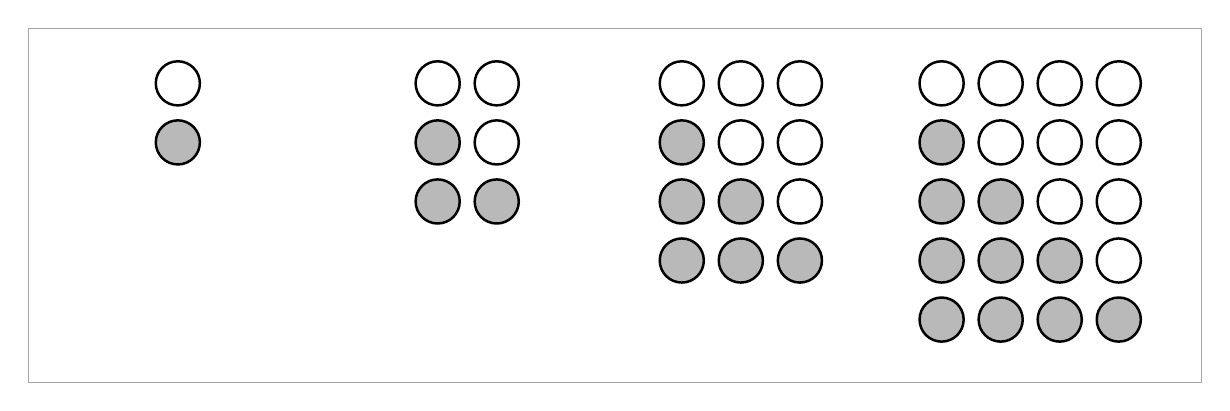
\begin{tikzpicture}[line cap=round,line join=round]
  % --- parameters ---
  \def\s{0.75}   % grid step
  \def\r{0.28}   % circle radius

  % --- outer frame ---
  \draw[gray!70] (-0.7,0.9) rectangle (14.2,-3.6);

  % styles
  \tikzset{
    odot/.style={draw=black,line width=.9pt},                 % empty circle
    gdot/.style={draw=black,fill=gray!55,line width=.9pt}     % filled circle
  }

  % helper: draw the (n columns) x (n+1 rows) block with staircase shading
  % rows are indexed from top (1) to bottom (n+1)
  \newcommand{\StairBlock}[1]{%
    \pgfmathtruncatemacro{\n}{#1}
    \pgfmathtruncatemacro{\m}{\n+1}
    \foreach \row in {1,...,\m}{%
      \foreach \col in {1,...,\n}{%
        % decide color: gray iff row>=2 and col <= row-1
        \pgfmathtruncatemacro{\gray}{(\row>=2) && (\col <= \row-1)}
        \ifnum\gray=1
          \filldraw[gdot] ({(\col-1)*\s},{-(\row-1)*\s}) circle (\r);
        \else
          \draw[odot] ({(\col-1)*\s},{-(\row-1)*\s}) circle (\r);
        \fi
      }%
    }%
  }

  % ========== (1) n=1 : 1x2 ==========
  \begin{scope}[shift={(1.2,0.2)}]
    \StairBlock{1}
  \end{scope}

  % ========== (2) n=2 : 2x3 ==========
  \begin{scope}[shift={(4.5,0.2)}]
    \StairBlock{2}
  \end{scope}

  % ========== (3) n=3 : 3x4 ==========
  \begin{scope}[shift={(7.6,0.2)}]
    \StairBlock{3}
  \end{scope}

  % ========== (4) n=4 : 4x5 ==========
  \begin{scope}[shift={(10.9,0.2)}]
    \StairBlock{4}
  \end{scope}
\end{tikzpicture}


\end{document}
